\documentclass[11pt]{article}

%% MinionPro fonts 
%\usepackage[lf]{MinionPro}
%\usepackage{MnSymbol}
\usepackage{microtype}

%% Margins
\usepackage{geometry}
\geometry{verbose,letterpaper,tmargin=1in,bmargin=1in,lmargin=1in,rmargin=1in}

%% Other packages
\usepackage{amsmath}
\usepackage{amsthm}
\usepackage[shortlabels]{enumitem}
\usepackage{titlesec}
\usepackage{soul}
\usepackage{tikz}
\usepackage{mathtools}
\usepackage{pgfplots}
\usepackage{tikz-3dplot}
\usepackage{algorithmic}
\usepackage[export]{adjustbox}
\usepackage{tcolorbox}
\usepackage{optprog}

%% Paragraph style settings
\setlength{\parskip}{\medskipamount}
\setlength{\parindent}{0pt}

%% Change itemize bullets
\renewcommand{\labelitemi}{$\bullet$}
\renewcommand{\labelitemii}{$\circ$}
\renewcommand{\labelitemiii}{$\diamond$}
\renewcommand{\labelitemiv}{$\cdot$}

%% Colors
\definecolor{rred}{RGB}{204,0,0}
\definecolor{ggreen}{RGB}{0,145,0}
\definecolor{yyellow}{RGB}{255,185,0}
\definecolor{bblue}{rgb}{0.2,0.2,0.7}
\definecolor{ggray}{RGB}{190,190,190}
\definecolor{ppurple}{RGB}{160,32,240}
\definecolor{oorange}{RGB}{255,165,0}

%% Shrink section fonts
\titleformat*{\section}{\normalsize\bf}
\titleformat*{\subsection}{\normalsize\bf}
\titleformat*{\subsubsection}{\normalsize\it}

% %% Compress the spacing around section titles
\titlespacing*{\section}{0pt}{1.5ex}{0.75ex}
\titlespacing*{\subsection}{0pt}{1ex}{0.5ex}
\titlespacing*{\subsubsection}{0pt}{1ex}{0.5ex}

%% amsthm settings
\theoremstyle{definition}
\newtheorem{problem}{Problem}
\newtheorem{example}{Example}
\newtheorem*{theorem}{Theorem}
\newtheorem*{bigthm}{Big Theorem}
\newtheorem*{biggerthm}{Bigger Theorem}
\newtheorem*{bigcor1}{Big Corollary 1}
\newtheorem*{bigcor2}{Big Corollary 2}

%% tikz settings
\usetikzlibrary{calc}
\usetikzlibrary{patterns}
\usetikzlibrary{decorations}
\usepgfplotslibrary{polar}

%% algorithmic setup
\algsetup{linenodelimiter=}
\renewcommand{\algorithmiccomment}[1]{\quad// #1}
\renewcommand{\algorithmicrequire}{\emph{Input:}}
\renewcommand{\algorithmicensure}{\emph{Output:}}

%% Answer box macros
%% \answerbox{alignment}{width}{height}
\newcommand{\answerbox}[3]{%
  \fbox{%
    \begin{minipage}[#1]{#2}
      \hfill\vspace{#3}
    \end{minipage}
  }
}

%% \answerboxfull{alignment}{height}
\newcommand{\answerboxfull}[2]{%
  \answerbox{#1}{6.38in}{#2} 
}

%% \answerboxone{alignment}{height} -- for first-level bullet
\newcommand{\answerboxone}[2]{%
  \answerbox{#1}{6.0in}{#2} 
}

%% \answerboxtwo{alignment}{height} -- for second-level bullet
\newcommand{\answerboxtwo}[2]{%
  \answerbox{#1}{5.8in}{#2}
}

%% special boxes
\newcommand{\wordbox}{\answerbox{c}{1.2in}{.7cm}}
\newcommand{\catbox}{\answerbox{c}{.5in}{.7cm}}
\newcommand{\letterbox}{\answerbox{c}{.7cm}{.7cm}}

%% Miscellaneous macros
\newcommand{\tstack}[1]{\begin{multlined}[t] #1 \end{multlined}}
\newcommand{\cstack}[1]{\begin{multlined}[c] #1 \end{multlined}}
\newcommand{\ccite}[1]{\only<presentation>{{\scriptsize\color{gray} #1}}\only<article>{{\small [#1]}}}
\newcommand{\grad}{\nabla}
\newcommand{\ra}{\ensuremath{\rightarrow}~}
\newcommand{\maximize}{\text{maximize}}
\newcommand{\minimize}{\text{minimize}}
\newcommand{\subjectto}{\text{subject to}}
\newcommand{\trans}{\mathsf{T}}
\newcommand{\bb}{\mathbf{b}}
\newcommand{\bx}{\mathbf{x}}
\newcommand{\bc}{\mathbf{c}}
\newcommand{\bd}{\mathbf{d}}

%% LP format
%    \begin{align*}
%      \maximize \quad & \mathbf{c}^{\trans} \mathbf{x}\\
%      \subjectto \quad & A \mathbf{x} = \mathbf{b}\\
%                       & \mathbf{x} \ge \mathbf{0}
%    \end{align*}


%% Redefine maketitle
\makeatletter
\renewcommand{\maketitle}{
  \noindent SA405 -- AMP \hfill Rader \#2.42 \\

  \begin{center}\Large{\textbf{\@title}}\end{center}
}
\makeatother

%% ----- Begin document ----- %%
\begin{document}
  
\title{HW5: Combinatorial Models Part 1}


\maketitle

% TSP

\textbf{Problem 1:} You are taking a trip to Busch Gardens and are a roller coaster enthusiast. There are 8 roller coasters at Busch Gardens: Pantheon (P), Griffon (G), Alpengeist (A), Tempesto (T), Lock Ness Mosnter (L), Apollo's Chariot (C), InvadR (I), and Verbolten (V). In order to expedite pedestrian flow, they have implemented several one way paths which make the distances between coasters non equidistant. Specifically, the table below gives the distance between each two coasters:

\begin{center}
\begin{tabular}{ccccccccc} 
  & P   & G   & A   & T   & L   & C   & I    & V  \\\hline
P & -   & 1.1 & 1.4 & 1.6 & 0.7 & 0.4 & 1.3  & 1.1 \\
G & 0.9 & -   & 0.7 & 1.1 & 0.3 & 2.1 & 0.5 & 1.9 \\
A & 1.2 & 0.6 & -   & 0.6 & 1.1 & 0.7 & 1.2 & 0.9 \\
T & 1.3 & 1.2 & 1.0 & -   & 1.0 & 1.2 & 0.8 & 0.6 \\
L & 0.5 & 0.2 & 0.8 & 0.9 & -   & 1.1 & 0.9 & 1.1 \\
C & 0.5 & 2.0 & 0.5 & 1.1 & 1.0 & -   & 0.7 & 1.1 \\
I & 1.5 & 0.7 & 1.1 & 0.9 & 1.1 & 0.9 & -   & 1.5 \\
V & 1.0 & 1.6 & 0.7 & 0.5 & 1.2 & 1.0 & 1.3 & - \\
\end{tabular}
\end{center}

Thus, for example, if you are walking from Pantheon to Tempesto, you are traveling 1.6 miles, but walking from Tempesto to Pantheon is a travel distance of 1.3 miles.

You want to ride each roller coaster while walking as little as possible.

\begin{enumerate}
\item[a.] Formulate a concrete model whose solution will give Cameron a tour that visits all 8 landmarks exactly once. \emph{Hint: Do not write all the subtour elimination constraints, you can write one or two then move on. Also, if you're having trouble getting started draw out the network for the problem.}
\item[b.] Convert your concrete model above to a parameterized model.
\item[c.] Suppose after solving your model, the solver returns the following solution. 

\verb|The following edges should be selected: (P,C), (G,P), (A,I), (T,A),| 

\verb|(L,G), (C,L), (I,V), (V,T)|
	\begin{enumerate}
	\item What are the values of your variables associated with this solution?
	\item What is the total distance traveled by this solution?
	\item Is this solution optimal for your TSP problem?
	\item If the solution is not optimal, write a constraint you could add to your model to remove this solution from your feasible region.
	\end{enumerate}
\end{enumerate}

\newpage

\textbf{Problem 2:} Another famous graph problem is the minimum spanning tree problem. A spanning tree is a tree which is connected to every node on the graph (with no cycles). This problem can be solved with an algorithm, but we can also solve it with integer programming.

A local phone company is interested in laying cable from the main road (where the
Main switch is located) to a new housing subdivision, and wants to do so in the least
expensive way.  It has the option of laying cable from the road to any house, or it can 
lay cable between the houses.  Each house must be connected through some path to 
the road.  The following matrix gives the total cost of laying cable between any two
locations, where the first location is the main road.

\begin{center}
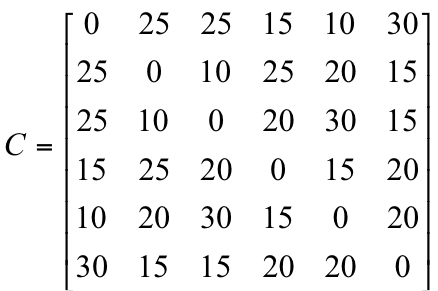
\includegraphics[width = .3\textwidth]{costs}
\end{center}

How should the phone company connect the houses to the road in order to minimize its
total cost?

\begin{enumerate}
\item[a.] How many edges should be a part of your spanning tree?
\item[b.] Formulate a concrete integer program which can be solved to find a minimum cost cable connection. \emph{Hint: There are three types of constraints in this model. One is given in part (a). What are the other two types of constraints we should include to get a connected tree?}
\end{enumerate}

\end{document}
